\chapter{PIP project}

\section{PIP protokernel}

\subsection{A minimal OS kernel with proovable isolation} \label{PIP}
An operating system is organized as a hierarchy  of layers, each one constructed  upon  the one  below  it. Each layer focuses on an essential role of the operating system such as memory management, multiprogramming, input/output \dots Generally speaking, while developping a kernel for an operating system based on the  layered  approach,  the designers have a choice where to draw the kernel-user boundary. Traditionally, all the  layers  went in the  kernel, but that is not necessary. In fact, putting as little as possible in kernel mode is safer because kernel bugs can bring down the system instantly. In contrast, user processes/layers are set up to have less power so that a bug there may not be fatal.\\

Various studies on bug density, relatively to the developped module size, age as well as other factors, have been conducted (e.g.  Basilli  and  Perricone in 1984;  and Ostrand  and  Weyuker in 2002). A  ballpark  figure  for  serious industrial systems is ten  bugs per thousand  lines  of code. Operating  systems  are  sufficiently  buggy  that  computer  manufacturers  put  reset  buttons  on  them, something  the  manufacturers of cars, TV sets and stereos do  not do,  despite  the  large  amount  of software in these devices. Furthermore, Operating systems generally present hardware resources to applications through high-level abstractions such as (virtual) file systems.\\

\noindent Therfore, there are several OS kernel families such as : 
\begin{itemize}
	\item \textbf{Microkernels :} The basic idea  behind a microkernel design  is  to  achieve  high reliability  by  splitting  the  operating  system  up  into  small,  well-defined  modules,  only  one  of  which, the  microkernel, runs  in  kernel  mode;
	\item \textbf{Exokernels :} The idea behind an exokernel is to force as few abstractions as possible on application developers, enabling them to make as many decisions as possible about hardware abstractions.
\end{itemize} 
  
\noindent Although the closest kernel design to PIP is the exokernel, PIP does not belong to any of the kernel families featured in the state of art, but it is the first member of a new kernel familiy, \textbf{protokernels}, as compared to most microkernels and exokernels, the TCB in PIP is even more restricted :
\begin{itemize}
	\item Scheduling and IPC are done in user mode unlike a microkernel;
	\item Multiplexing is also done in user mode unlike an exokernel.
\end{itemize}

\noindent Whereas the kernel mode is only for \textbf{multi-level MMU conguration} (virtual memory) and \textbf{context switching}. This not only ensures less bugs density but also more feasibility of formal proof that will warrant the memory isolation property of the protkernel. \\

As a \textbf{minimal OS Kernel with provable isolation}, PIP focuses more on security and safety without sacrificing efficency and ensures memory isolation between different tasks running on the same device.PIP's algorithmic part is written in Gallina, the language of the Coq proof assistant, in a monadic style that allows direct translation into freestanding C. We will refer to this implementation in Gallina as the shallow embedding in contrast to the deep embedding introduced in section \ref{deep} p.\pageref{deep}. 

\begin{figure}[!ht]
	\centering 
	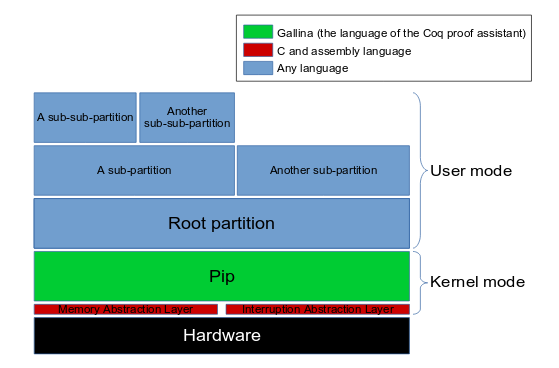
\includegraphics[width=\linewidth ,frame]{img/OSLayersPIP.png} 
	\caption{Software layers of an OS built on top of PIP}
\end{figure}

\subsection{Horizontal isolation \& vertical sharing}

PIP can be used to partition the available memory which will be initially allocated to the root partition on top of PIP. Any partition can read and write in the memory of its children. However, partitions in diffrent branches of the partition tree are disjoint. The former is referred to as \textbf{vertical sharing} and the latter as \textbf{horizontal isolation}. Needless to say, all memory lended to PIP for storing kernel data, when creating partitions for exemple, are inaccessible for all partitions to prevent messing up PIP data structures which means that the kernel data is totally isolated.
   
\begin{figure}[!ht]
	\centering 
	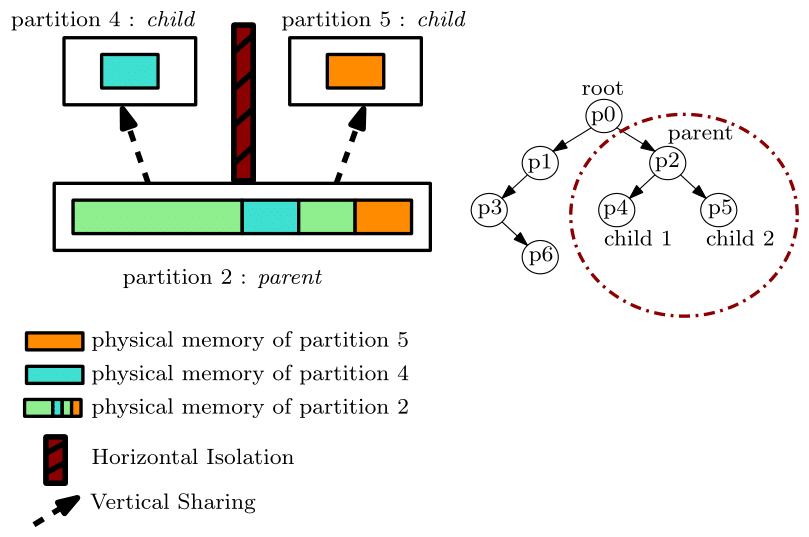
\includegraphics[width=0.8\linewidth,frame]{img/memoryIsolShare.png} 
	\caption{Horizontal isolation \& vertical sharing in PIP}
\end{figure}

\noindent If we consider a more realistic partition tree as shown in figure \ref{FreeRTOS} in which we consider Linux and FreeRTOS as sub-partitions of a root partition, multiplexer. Knowing that FreeRTOS is a real-time OS that does not isolate its tasks, we easily secured it with task isolation by porting it on PIP.

\begin{figure}[!ht] \label{FreeRTOS}
	\centering 
	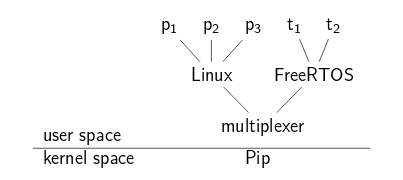
\includegraphics[scale=0.5,frame]{img/FreeRTOSEx.png} 
	\caption{FreeRTOS task isolation using PIP}
\end{figure}

\subsection{Proof oriented design}
PIP's isolation properties are meant to be formally prooved independently of the platform it's running onto. Consequently, the algorithm and the architecture dependant part were separated. Indeed, as shown in figure \ref{design}, PIP is splitted into two distinct layers  :
\begin{itemize}
	\item \textbf{HAL :} gives direct access to the architecture and hardware;
	\item \textbf{API :} implements the algorithmic part to configure the virtual memory and the hardware.
\end{itemize}

\noindent The API code is written and proven using the Coq proof assistant, and uses the interface provided by the HAL to perform any hardware related operation. the proofs are based on Hoare logic theory introduced in section \ref{Hoare} p.\pageref{Hoare}.

\begin{figure}[!ht]  
	\centering 
	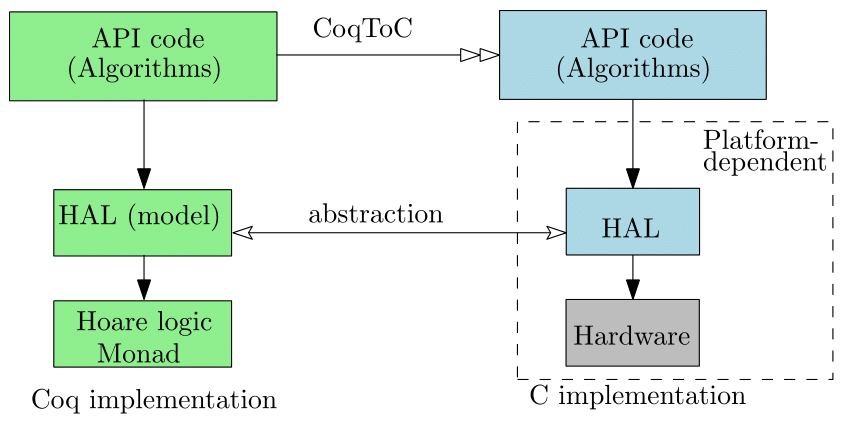
\includegraphics[width=0.8\linewidth, frame]{img/PIPDesign.png} 
	\caption{PIP design}
	\label{design}
\end{figure}

\noindent PIP's HAL is splitted into three components, as shown in figure \ref{HAL}, each handling a specific part of the target platform's hardware :
\begin{itemize}
	\item \textbf{Memory Abstraction Layer (MAL) :} provides an interface for the configuration of the MMU chip;
	\item \textbf{Interrupt abstraction Layer (IAL) :} provides an iterface to dispatch interrupts and configure hardware;
	\item \textbf{Bootstrap :} contains the low-level code required to boot the system.
\end{itemize}

\noindent PIP only provides system calls for management of partitions and for context switching, thus reducing the TCB to its bare minimum as explained in section \ref{PIP} p.\pageref{PIP}. This user exposed API can be called by any partition using a platform dependant call :
\begin{itemize}
	\item \textbf{createPartition :} creates a new child (sub-partition) into the current partition;
	\item \textbf{deletePartition :} removes a child partition and puts all its used pages back in the current partition;
	\item \textbf{prepare :} adds required configuration tables into a child partition to map a new virtual address;
	\item \textbf{collect :} removes the empty configuration tables which are not used anymore and gives it back to the current partition; 
	\item \textbf{countToMap :} returns the amount of configuration tables needed to perform a mapping for a given virtual address;
	\item \textbf{addVaddr :} maps a virtual address into the given child;
	\item \textbf{removeVAddr :} removes a given mapping from a given child.
\end{itemize} 
This API is sufficient as far as memory requirements are concerned but it lacks a way to handle interrupts. Hardware interrupts are implicitly handled by PIP and automatically dispatched to the root partition, while software interrupts, such as system calls, are notified to the partent partition of the caller and can be managed by these two additional services of PIP :
\begin{itemize}
	\item \textbf{dispatch :} notifies an interrupt to a given partition, interrpting its current control flow and backing it up for a further resume call;
	\item \textbf{resume :} restores a previously interrupted context.
\end{itemize} 

\begin{figure}[!ht]  
	\centering 	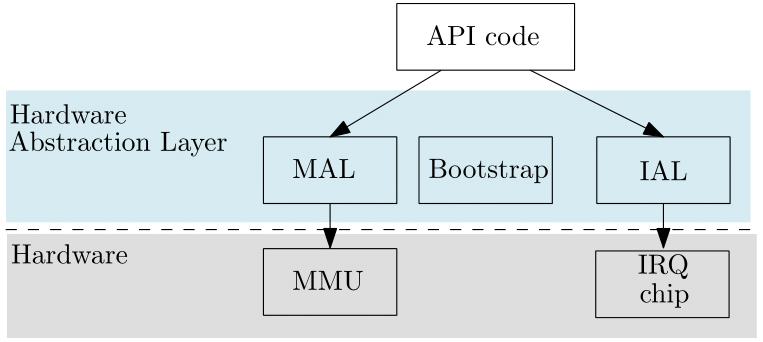
\includegraphics[width=0.8\linewidth,frame]{img/HAL.png} 
	\caption{HAL and API relationship}
	\label{HAL}
\end{figure}

\subsection{More In depth understanding of PIP's Data structures}

\subsubsection{The memory}

PIP uses several data stuctures per partition, which will represent the global state of the partition's memory state. This is necessary as it has to keep track of pages allocated to partitions in order to allow or deny derivation and partition creation while preserving the required properties. \\

Figure \ref{partitionEx} shows a partition tree example consisting of a  partition, Parent, that has a single child, Child1. A partition is identified by a partition descriptor which a page number essentiel to access the whole data structure of a partition. In our case, the partition descriptors of Parent and Child1 are respectively 1 and 12. The pages lent to PIP to manage a partition are organized in a tree with three branches : the MMU tables, the first shadow and the second shadow. The aim of this organization is to keep additional information about each page lent to a partition. Moreover these structures have multiple goals :
\begin{itemize}
	\item \textbf{Access control :} the first shadow is used to avoid derivating the same page multiple times;
	\item \textbf{Performance :} the second shadow and the configuration list are used to quickly find the virtual address of a page without having to parse the whole virtual space when the parent partition reclaims it.
\end{itemize} 
As such, adding an indirection table in the MMU configuration requires two additional pages for the shadows. Therefore, this model is estimated to require roughly thre times the amount of memory a simple virtual environment would need, but it provides nevertheless a both secure and efficient API. \\

To proove the isolation properties on this memory structure it is essentiel to assure it's consistency relative to the partition tree, the well typedness as well as some other consistency properties that will be detailed in section \ref{Hoare} p.\pageref{Hoare}.

\vfill 

\begin{figure}[!ht]  
	\centering 
	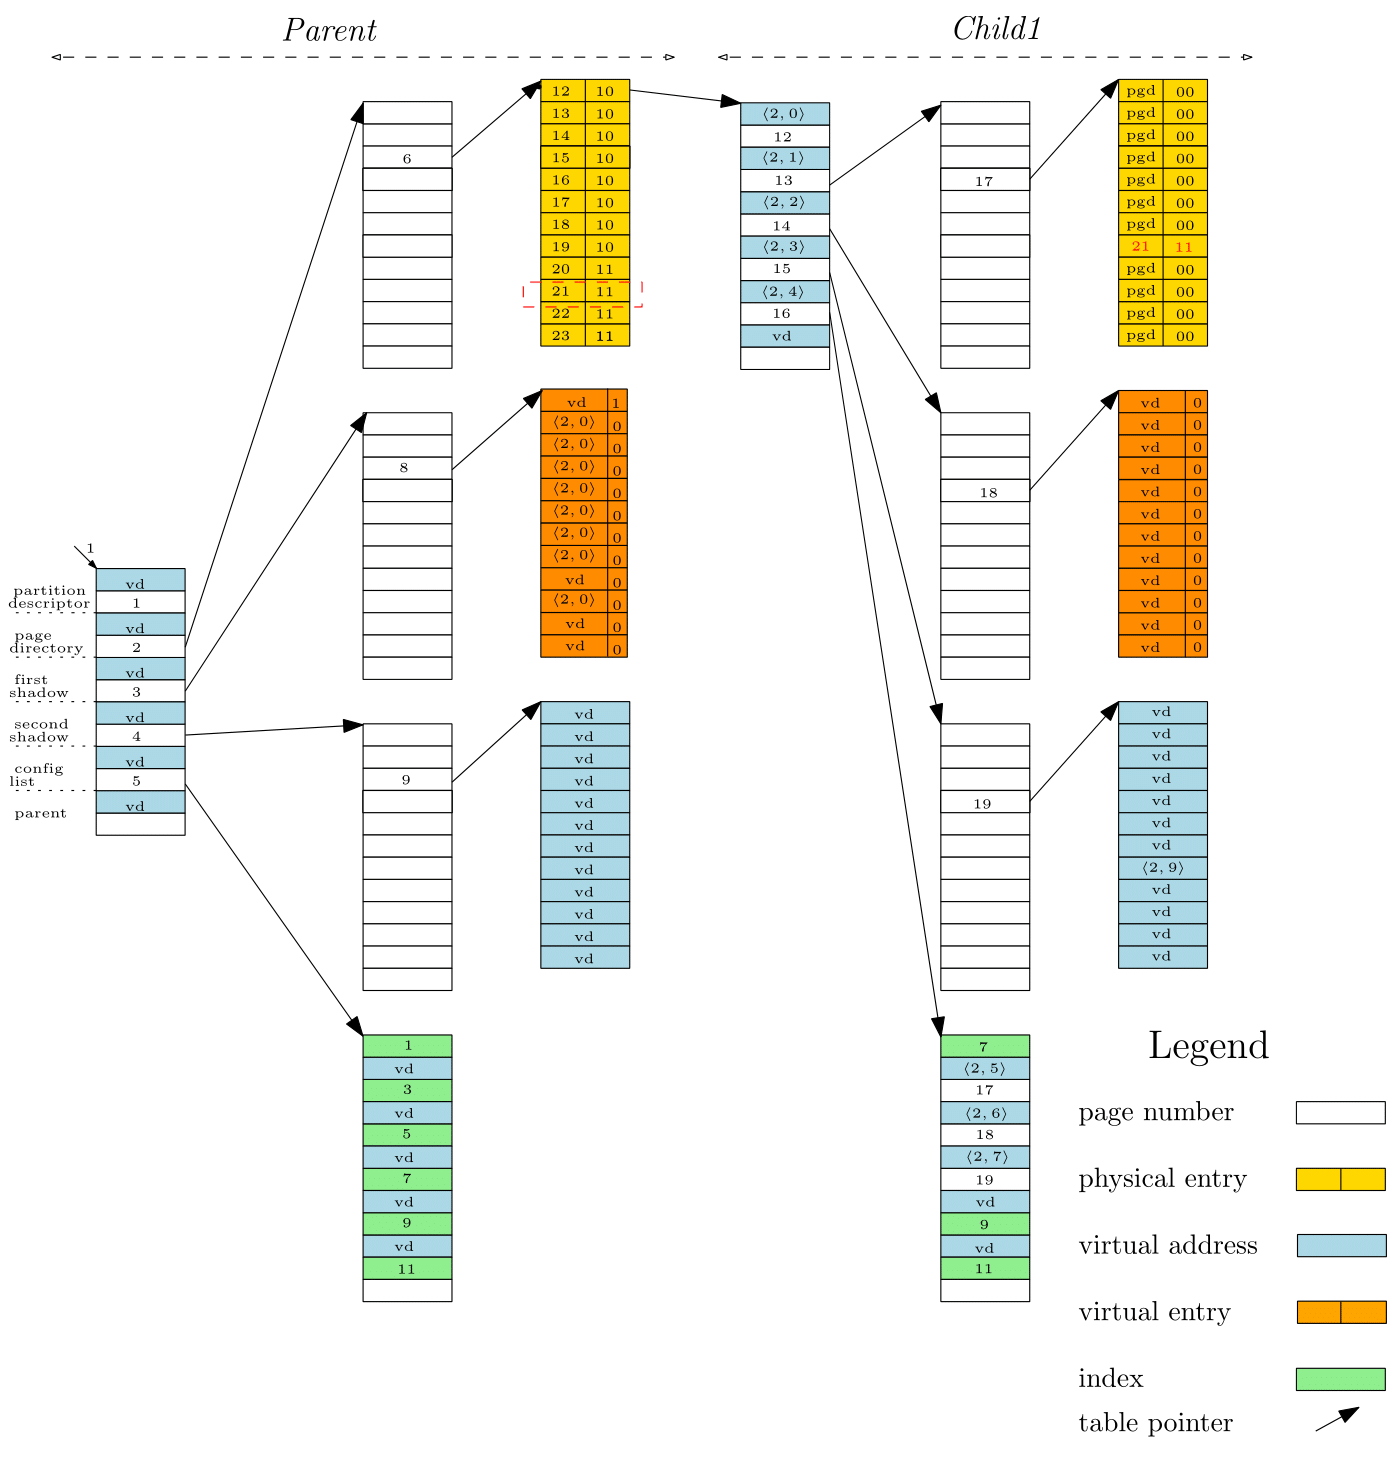
\includegraphics[width=1\linewidth, height=0.6\textheight, frame]{img/memoryEx.png} 
	\caption{An example of a partition tree}
	\label{partitionEx}
\end{figure}

\subsubsection{The state}
 
\noindent The PIP state is defined as follows :
\begin{lstlisting}[caption = {PIP state definition}] 
Record state : Type := 
{ currentPartition: page ; memory: list (paddr * value) }.
\end{lstlisting}
The list in the state corresponds to the physical memory and maps physical addresses to values.A physical address is defined by a physical page number and a position into this page :
\begin{lstlisting}[caption = {paddr type definition}] 
	    Definition paddr := page * index.
\end{lstlisting}
where pages and indexes are positive integers bounded respectively by the overall number of pages and the table size :
\begin{lstlisting}[caption = {page \& index type definitions}]
Record page := { p :> nat ; Hp : p < nbPage }. 
Record index := { i :> nat ;  Hi : i < tableSize }.
\end{lstlisting}
Different types of values could be stored into the physical memory by Pip so the type value is an inductive type defined as follows :
\begin{lstlisting}[caption = {value type definition}]
		Inductive value : Type:=
		| PE: Pentry -> value
		| VE: Ventry -> value
		| PP: page   -> value
		| VA: vaddr  -> value
		| I:  index  -> value.
\end{lstlisting}
The type Pentry which represents a phisical entry consists of a physical page number along with several flags :
\begin{lstlisting}[caption = {Pentry type definition}]
		Record Pentry : Type:= {
  		 read:    bool ;
   		 write:   bool ;
   		 exec:    bool ;
   		 present: bool ;
   		 user:    bool ;
   		 pa:      page }.
\end{lstlisting}
Finally, the \textit{Ventry} type consists of a virtual address with a unique bolean flag :
\begin{lstlisting}[caption = {Ventry type definition}]
Record Ventry : Type:= { pd: bool ; va: vaddr }.
\end{lstlisting}
with virtual addresses modeled as a list of indexes of length the number of levels of the MMU plus one :
\begin{lstlisting}[caption = {vaddr type definition}]
Record vaddr : Type := 
{ va :> list index ; Hva : length va = nbLevel + 1  }.
\end{lstlisting}

\section{Hoare logic} \label{Hoare}

\subsection{Introduction to Hoare logic theory}
\textit{How can we argue that a program is correct ?}
Nowadays, Building reliable software is becoming more and more difficult considering the growing scale, specifications and complexity of modern systems. Therefore, tests alone can no longer ascertain the reliability of programs especially if we're talking about critical systems. Logicians, computer scientists and software engineers have responded to these challenges by developing different kinds of techniques some of which are based on formal reasoning about properties of software and tools for helping validate these properties. One of these reasoning techniques that was used to proove PIP's properties is \textit{Floyd–Hoare logic}, often shortened to just \textbf{Hoare Logic}. It was proposed in 1969 by the British computer scientist and logician Tony Hoare and it continues to be the subject of intensive research right up to the present day. It is not only a natural way of \textbf{writing down specifications of programs} but also a technique for \textbf{proving that programs are correct} with respect to such specifications.\\

Let S be a Program that we want to execute starting from a certain state s, P a predicate on the state describing the condition S relies on for correct operation and Q a predicate on the resulting state after the execution of S describing the condition S establishes after correctly running. Knowing that P is verified on s, if we proove that Q is verified after the execution of s, we can ascertain that S is partially correct. And by partial correctness of S we mean that S is correct if it terminates. Using standard Hoare logic, only partial correctness can be proven, while termination needs to be proved separately. This triple S, P and Q, written as \textbf{ \{P\} S \{Q\} }, is referred to as a \textbf{Hoare triple}. The assertions P and Q are respectively referred to as the \textbf{precondiction} and the \textbf{postcondition}. \\

\noindent For example let's consider simple Hoare triples about an assignment command :
\begin{itemize}
	\item \boldmath$\{X=2\} X:=X+1 \{X=3\}$ : is a valid Hoare triple, that can be easily formally prooved in Coq, since the postcondiction is verified after the execution of the assign command relatively to the precondition;
	\item \boldmath$\{X=2\} X:=X*2 \{X=3\}$ : is not a valid Hoare triple since the postcondition would not be verified after the execution of the command.
\end{itemize} 

\pagebreak

\noindent Now, let's introduce some facts and rules about Hoare triples :
\begin{enumerate}
\item If an assertion P implies another precondition P' of a valid Hoare triple \{P'\} S \{Q\} then \{P\} S \{Q\} is also a valid Hoare triple. This is referred to as \textbf{weaking the precondition of a Hoare triple} and can be formally defined as follows :
\begin{center}
$\forall$ S P P', (P $\rightarrow$ P') $\rightarrow$ \{P'\} S \{Q\} $\rightarrow$ \{P\} S \{Q\}
\end{center}
\item If we can weaken a Hoare triple, we expect it to have a \textbf{weakest precondition}. This notion was introduced by Dijkstra in 1976 and is very important since it enables us to proove total correctness and in particular program termination. Indeed, if a program doesn't terminate, its weakest precondition would be \textit{True} and it would verify any postcondition.
\item If we consider a language containing a \textbf{SKIP instruction} which practically does nothing, we can affirm that this command preserves any property which means :
\begin{center}
$\forall$ P, \{P\} SKIP \{P\}
\end{center}
\item If we consider a language that allows \textbf{assingments}, in the form of \linebreak X := a, then we can conlude that an arbitrary property Q holds after such assignment if we assume Q[X$\rightarrow$a] which means Q with all occurences of X replaced by a :
\begin{center}
$\forall$ Q X a, \{Q[X$\rightarrow$a]\} X:= a \{Q\}
\end{center}
\item Generally speaking, every Program is built using \textbf{sequencing} of commands that we will write as C1\textbf{;}C2. Our aim is to proove a Hoare triple on this sequence with P and Q respectively as the precondition and the postcondition of this triple. This requires prooving that C1 takes any state where P holds to a state where an intermediate assertion I holds and C2 takes any state where I holds to one where Q holds  which could be formally stated as :
\begin{center}
$\forall$ P I Q C1 C2, \{P\} C1 \{I\} $\rightarrow$ \{I\} C2 \{Q\} $\rightarrow$
\{P\} C1\textbf{;}C2 \{Q\}
\end{center}

\end{enumerate} 


%formal definition of these properties
%https://www.cs.cmu.edu/~aldrich/courses/654-sp07/slides/7-hoare.pdf

\section{Verification of invariants in the shallow embedding}

\section{The deep embedding} \label{deep}

\section{Hoare logic in the deep embedding}